\documentclass{../source/Experiment}

\major{信息工程}
\name{}
\title{直方图计算与均衡化}
\stuid{}
\college{信息与电子工程学院}
\date{\today}
\lab{}
\course{数字图像处理}
\instructor{李东晓}
\grades{}
\expname{直方图计算与均衡化}
\exptype{设计验证}
\partner{}
\begin{document}
\makecover
\section{实验任务}
本次选择的是PROJECT-03-02题目。

\bfseries{直方图均衡化}

\begin{enumerate}
    \item 编写一个程序计算一个图像的直方图。
    \item 利用3.3.1节讨论的公式执行直方图均衡化操作。
    \item 对一张图片实现直方图均衡化。
\end{enumerate}
\section{算法设计}
\subsection{直方图计算}
令$r_k, k = 0,1,2,...,L-1 $表示一幅$L$级灰度数字图像$f(x,y)$的灰度,则$f$的非归一化直方图定义为
$$h(r_k) = n_k, k = 0,1,2,...,L-1$$
式中,$n_k$是$f$中灰度为$r_k$的像素的数量。
$f$的归一化直方图定义为
$$p(r_k) = \frac{h(r_k)}{MN} = \frac{n_k}{MN}$$
式中,$M$和$N$分别表示图像的行数和列数。

编程时,我们可以先统计出图像的灰度取值,然后遍历图像的所有像素,对不同灰度值进行计数,统计出所有灰度值对应的像素个数,画出统计频次对于灰度值的直方图,即可得到非图像的非归一化的直方图。同时可以计算出不同灰度值的频次,画出归一化的直方图。
\subsection{直方图均衡化}
对于离散的灰度值,可以用概率求和代替概率密度函数与积分,得到变换后的$s_k$为

$$sk = T(r_k) = (L - 1)\sum^k_{j = 0}p_r(r_j), \quad k = 0,1,2,...,L-1$$

编程时可以利用上式进行直方图均衡化,同时对于计算出的值进行四舍五入取整作为变换后的灰度值。
\section{代码实现}
本次实验编程语言选择的是Matlab。

计算图像的直方图信息核心代码如下:

\begin{lstlisting}[language = matlab]
    % 获取灰度直方图的信息(r,数量,概率)
    [Y,X] = size(img_gray);
    grayvalue = unique(img_gray);
    l = 256 - length(grayvalue);
    b = zeros(l, 1);
    grayvalue = cat(1,grayvalue,b);
    imginfo=[];
    for i=1:length(grayvalue)
            [ANSy,ANSx]=find(img_gray==grayvalue(i));
            imginfo.gray(i)=grayvalue(i);
            imginfo.count(i)=length(ANSy);
            imginfo.prob(i)=length(ANSy)/(Y*X);
    end 
        \end{lstlisting}
其中,imginfo类中的gray保存了图像的灰度值,count保存了各个灰度值的频次统计,prob保存了各个灰度值的频率统计。

实现直方图均衡化的核心代码如下:
\begin{lstlisting}[language = matlab]
    % 获取量化后的灰度s,数量,概率
    hist_eq = [];
    hist_eq.gray = imginfo.gray;
    hist_eq.s = zeros(1,256);
    hist_eq.round_s = zeros(1,256);
    hist_eq.count = zeros(1,256);
    for k = 1:1:length(grayvalue)
        for j = 1:1:k
            hist_eq.s(k) = hist_eq.s(k) + imginfo.prob(j);
            hist_eq.count(k) = hist_eq.count(k) + imginfo.count(j);
        end
        hist_eq.s(k) = (255) * hist_eq.s(k);
    end
    hist_eq.round_s = round(hist_eq.s);
        \end{lstlisting}
其中,hist\_eq类中gray保存了均衡化之前的灰度值,s保存了均衡化之后的灰度值(未四舍五入),round\_s保存了四舍五入后的s值,count保存了均衡化后的灰度值的频次。

获取均衡化后的图像核心代码如下:
\begin{lstlisting}[language = matlab]
    % 获取均衡化后的图像
    imgHist = zeros(size(img_gray));
    for y = 1:1:Y
        for x = 1:1:X
            i = img_gray(y,x);
            imgHist(y,x) = hist_eq.round_s(i+1);
        end
    end
    imgHist = uint8(imgHist);
        \end{lstlisting}
其中imgHist为均衡化后的图像二维矩阵。

实验完整代码附录。
\section{实验结果}
实验测试图像使用如下图像:
\begin{figure}[H]
    \centering
    
\includegraphics[width = 0.6\textwidth]{第一次/aini.jpg}
    \caption{测试图像}
\end{figure}

通过自己编写的计算直方图的程序得到的结果如下,同时与Matlab自带的计算直方图函数imhist()比较,可以看出两者几乎没有差别,也看出原始图像的灰度主要集中在灰度低的地方,灰度高的地方几乎没有会度分布,原图的灰度图偏暗,对比度低。
\begin{figure}[H]
    \centering
    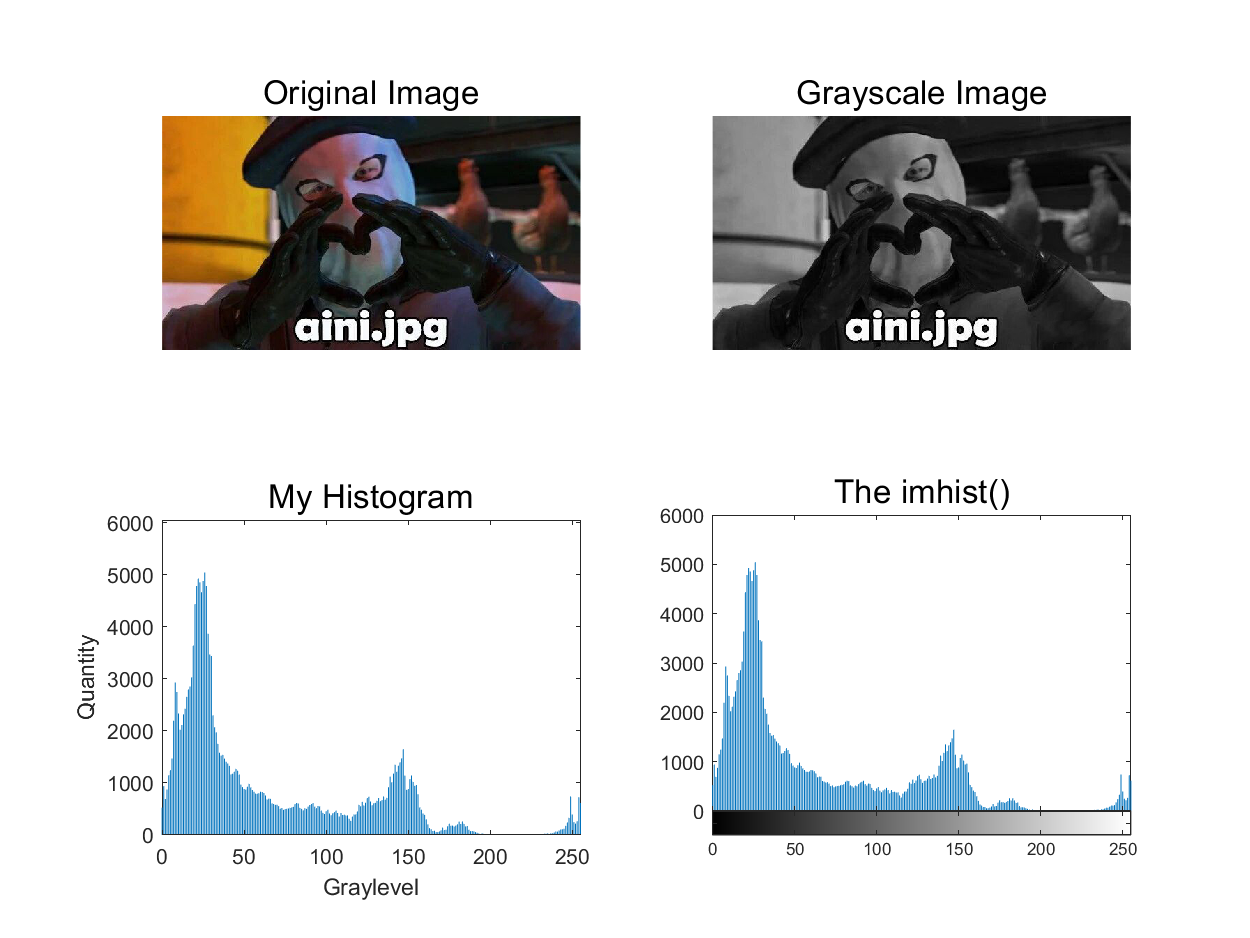
\includegraphics[width = 0.9\textwidth]{第一次/hw1-1.png}
    \caption{直方图计算结果}
\end{figure}

直方图均衡化后得到的直方图结果以及$s-r$函数如下,可以看出经过直方图均衡化后,原本灰度低的地方分布变得分散,而灰度高的地方有了较为均匀的灰度分布。
\begin{figure}[H]
    \centering
    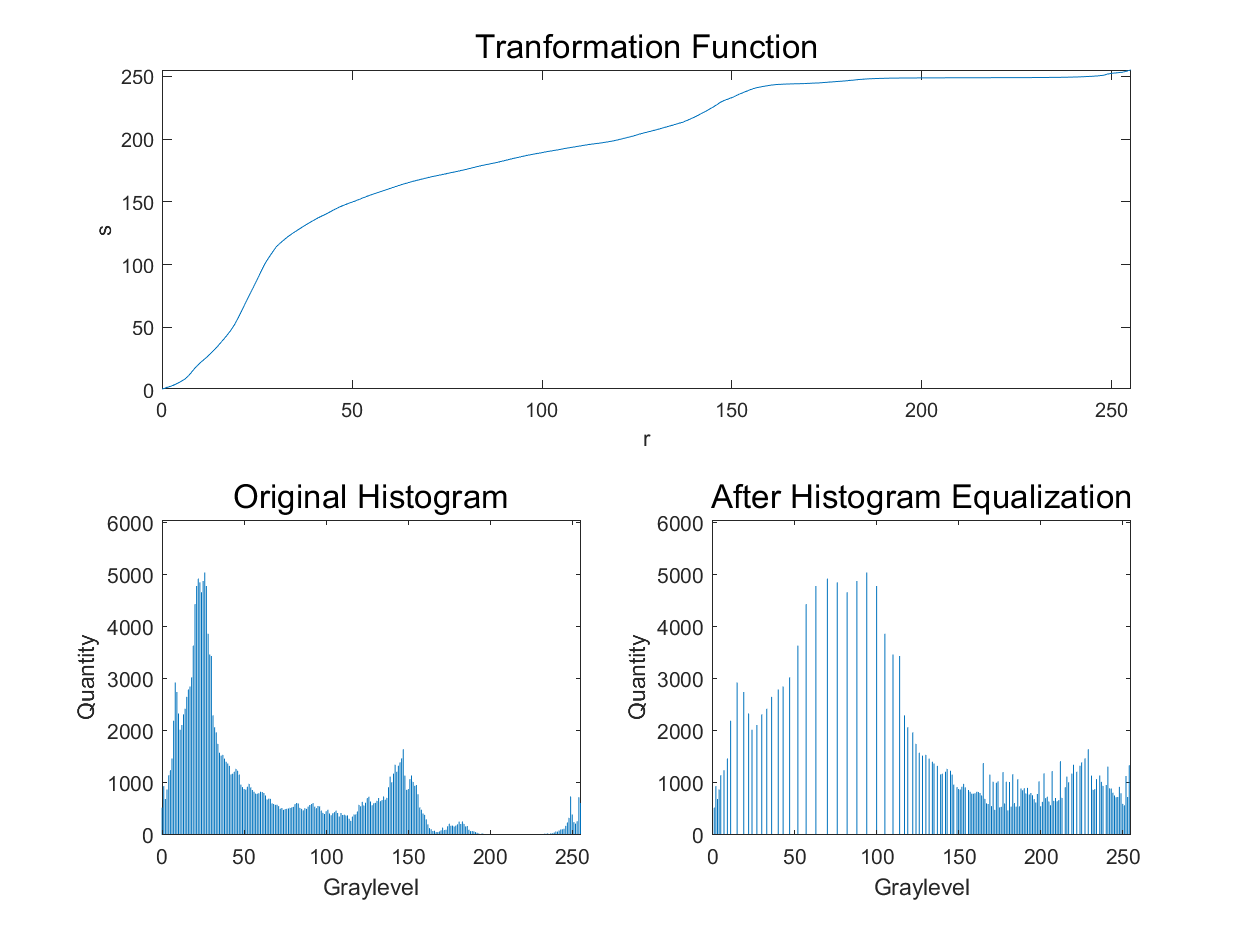
\includegraphics[width = 0.9\textwidth]{第一次/hw1-2.png}
    \caption{均衡化后直方图结果}
\end{figure}

对比均衡化之前的灰度图像可以看出,均衡化之前图像偏暗,对比度较低;均衡化之后图像整体变亮,对比度提高。

\begin{figure}[H]
    \centering
    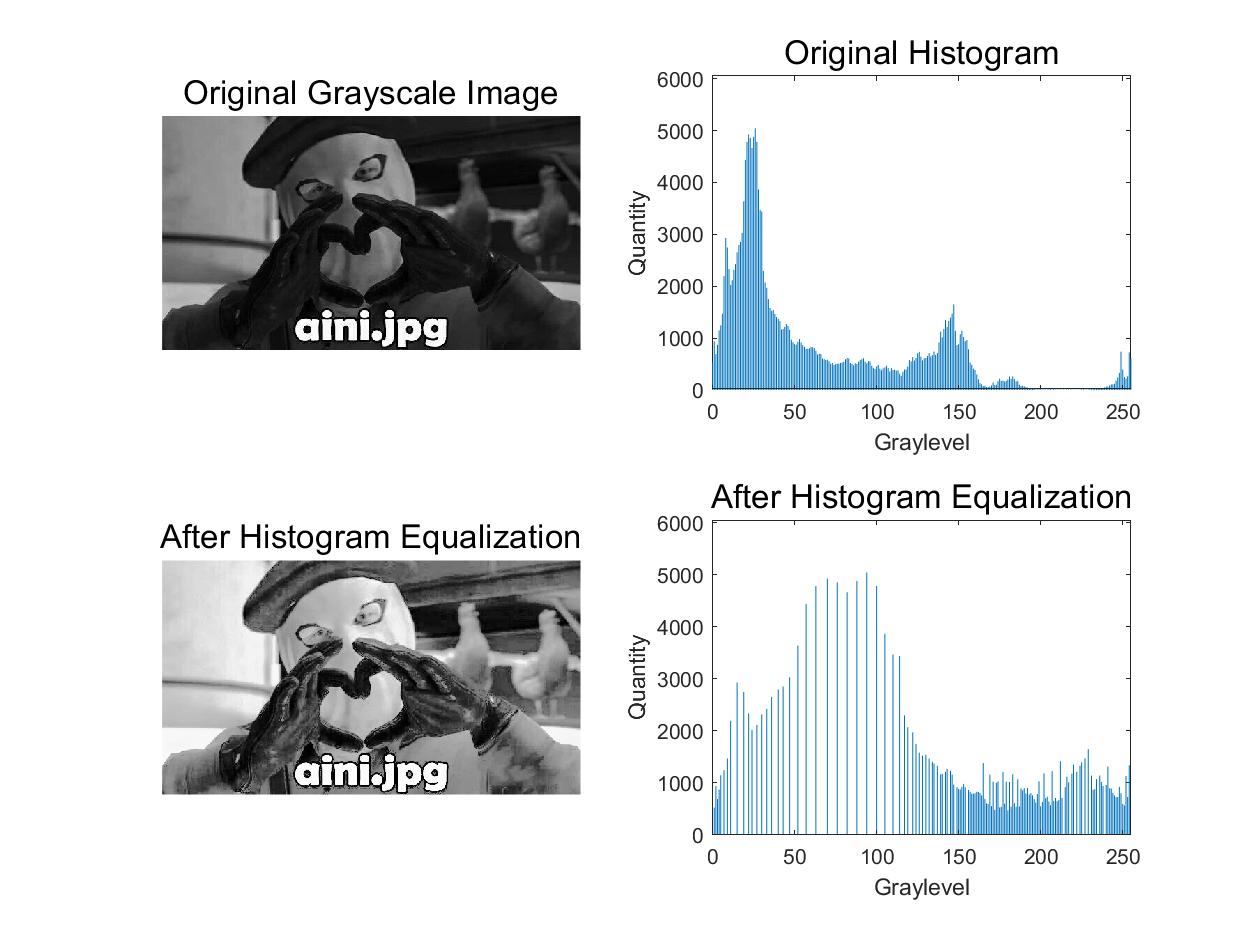
\includegraphics[width = 0.9\textwidth]{第一次/hw1-3.png}
    \caption{均衡化前后灰度图对比}
\end{figure}

最后将自己的直方图均衡化结果与Matlab自带的均衡化函数histeq()进行对比,从直方图可以看出自己的均衡化效果还不及Matlab自带的函数,仍有改进空间,结合已经学内容,可以通过直方图规定化进行一定的改进。
\begin{figure}[H]
    \centering
    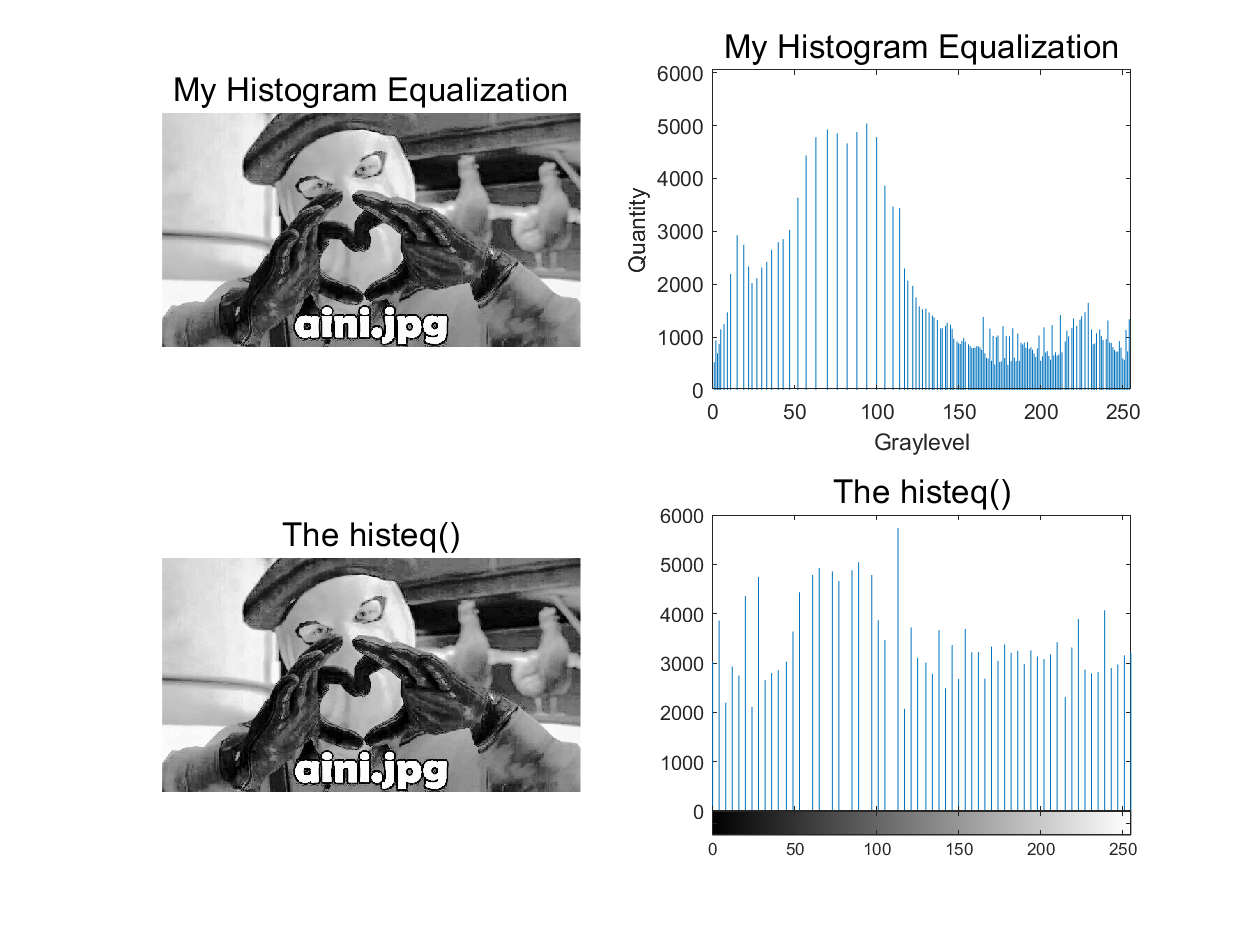
\includegraphics[width = 0.9\textwidth]{第一次/hw1-4.png}
    \caption{直方图计算结果}
\end{figure}

\section{总结}
本次实验主要是通过Matlab编程语言实现了课程中所讲的灰度图的直方图计算绘制以及直方图均衡化。

在实验的过程中,我对于课程中所学的直方图以及均衡化的理论有了更加深刻的理解,同时也意识到课程中所讲的内容与实际应用还有一定的差别,需要更多的理解与学习。

\section{附录:实验完整代码}
\lstinputlisting[
    language  =   matlab
]{第一次/homework1.m}

\end{document}


